\documentclass[10pt, compress]{beamer}
\usetheme[conference=MST1-GPM,venue=Garching, date=15/11/2016, titleprogressbar, logo=RFX-logo]{Eurof}
\usepackage{listings,amsmath,multimedia, amssymb}
\usepackage{../beamerclass/tangocolors}
\usepackage{../beamerclass/rfxcolor}
% for drawing
\usepackage{pgf}
\usepackage{tikz}
\usetikzlibrary{arrows,shapes,backgrounds}
\usepackage{../beamerclass/onimage}
\usepackage[export]{adjustbox}
\usepackage{bm}
% for font
\usepackage[absolute,overlay]{textpos}
  \setlength{\TPHorizModule}{1mm}
  \setlength{\TPVertModule}{1mm}

\usepackage[style=nature,citestyle=authoryear-comp,defernumbers=true,maxnames=2,firstinits=true,
uniquename=init,backend=bibtex8,arxiv=abs,mcite]{biblatex}
\bibliography{biblio}
\renewcommand*{\bibfont}{\footnotesize}
\renewcommand*{\citesetup}{\footnotesize}
\usepackage[export]{adjustbox}
\makeatother
\mode<presentation>
\makeatletter
% add a macro that saves its argument
\newcommand{\footlineextra}[1]{\gdef\insertfootlineextra{#1}}
\newbox\footlineextrabox
% for reducing font on a single slide
\newcommand\Fontvi{\fontsize{8}{7.2}\selectfont}
\title{Filamentary transport in high-power H-mode conditions and in
  no/small-ELM regimes to predict heat and particle loads on PFCs for
  future devices}
\date{15 November 2016}
\author[Topic 21. J. Madsen and N.Vianello]{J. Madsen and N. Vianello}
\begin{document}
\tikzstyle{every picture}+=[remember picture]
\maketitle

\begin{frame}{Main focus of topic 21 is shoulder formation}
\vspace{-1cm}
Objectives:
\begin{enumerate}
\item Use the new HHF probe on AUG to study filamentary transport under
high-power H-mode conditions and under different plasma configurations (SN,
DN).
\item Study the role of ELM regimes, neutral compression, and particle density in
filamentary transport and related shoulder formation.
\item Identify the contribution of collisionality and seeding on filamentary transport
and related shoulder formation.
\item Extend the studies to quiescent H-modes as well as to other small-ELM regimes.
\item Determine the effect of filaments and shoulder formation on target heat loads
in different H-mode plasmas.
\item Investigate the effect of plasma shape and configuration on ELM-induced heat
loads.
\end{enumerate}
\underline{Motivation}: Particle and energy transport in the SOL is crucial for the lifetime of plasma facing components in ITER and DEMO
\end{frame}

\section{Background}
\begin{frame}{Present status}
  \setbeamercovered{transparent}
  \begin{enumerate}[<+(1) | invisible@-+>]
    \item Experimental and theoretical investigations suggest that SOL density profiles are  determined by the balance between radial filamentary transport and parallel dynamics
    \item The balance changes at high density and leads to broadened SOL density profiles $\rightarrow$ \emph{shoulder formation}
    \item This is observed in L-mode plasmas in a variety of devices including AUG \parencite{Carralero:2014gs},
      TCV \parencite{Garcia:2007p2615} and MAST \parencite{Militello:2016hk}
    \item Observations exhibit various dependencies on divertor
      collisionality, plasma current,  seeding. \alert{Results from
        different devices not fully reconciled and the underlying mechanism is not fully understood.}
    \item Studies of shoulder formation in H-Mode are so far limited 
	%\item Particle and energy transport in the SOL is crucial for lifetime of PFC in ITER and DEMO
%    \item First we will report a summary of the achievements and then
 %    personal comments and plans
    \end{enumerate}
\end{frame}
\section{L-Mode}
\begin{frame}{L-Mode studies: AUG/1}
  \begin{columns}
    \begin{column}{0.5\textwidth}
      \begin{itemize}
      \item<1-> AUG and JET \parencite{Carralero:2015gu} suggest that
        \begin{equation*}
        \Lambda_{div} = \frac{L_{\parallel}/c_s}{1/\nu_{ei}}\frac{\Omega_i}{\Omega_e}
      \end{equation*}
      controls shoulder formation
        \item<2-> \textcolor{red}{Tested by changing n$_e$
            and $T_e$ through fueling/seeding/heating}
        \item<3-> This determines a change of the velocity-size
          scaling from
        \textcolor{ta3chameleon}{sheath-limited}
        to \textcolor{blue}{inertial regime}. \onslide<4>{\alert{$\Lambda_{div}$ rules the density profile scale
          length}} 
        \end{itemize}
    \end{column}
    \begin{column}{0.5\textwidth}
      \only<1-2>{
      \begin{tikzonimage}[width=\textwidth]{../pdfbox/KoM15Nov/CarraleroPRL15a}
          \draw [thick, ta3chameleon, thick, rotate=1] (0.43,0.25) ellipse (0.23 and 0.1);
          \draw [thick, blue, thick, rotate=-4] (0.8,0.55) ellipse (0.1 and 0.33);
        \only<2>{
          \draw [ultra thick, red, thick, dashed] (0.5,0.63) circle (0.12);
        }
      \end{tikzonimage}}
    \only<3>{
      \begin{tikzonimage}[width=\textwidth]{../pdfbox/KoM15Nov/CarraleroPRL15b}
          \draw [ultra thick, ta3chameleon, rotate=1] (0.2,0.5) ellipse (0.05 and 0.4);
          \draw [thick, blue, rotate=15] (0.65,0.07) ellipse (0.4 and 0.1);
      \end{tikzonimage}
    }
    \includegraphics<4>[width=\textwidth]{../pdfbox/KoM15Nov/CarraleroPRL15c}
    \end{column}
  \end{columns}
\end{frame}
\begin{frame}{L-Mode studies: AUG/2}
  \begin{columns}
    \begin{column}{0.5\textwidth}
      \begin{itemize}
      \item<1-> Profile modified by increase of blob-size and change of
        \alert{packing fraction: $f_{fil} = \nu_{fil}\tau_{AC}$}
        \onslide<2->{\textcolor{blue}{and filament relative density}
          {\footnotesize (Carralero 2016 in preparation)}}
      \item<3-> As a consequence the contribution of filaments to
        radial transport increases
      \item<4> Parallel flow is strongly reduced whenever we increase
        the divertor collisionality
      \end{itemize}
    \end{column}
      \begin{column}{0.5\textwidth}
        \includegraphics<1>[width=\textwidth]{../pdfbox/KoM15Nov/CarraleroMST16a}
        \includegraphics<2>[width=\textwidth]{../pdfbox/KoM15Nov/CarraleroMST16b}
        \includegraphics<3>[width=\textwidth]{../pdfbox/KoM15Nov/CarraleroMST16c}
        \includegraphics<4>[width=\textwidth]{../pdfbox/KoM15Nov/CarraleroMST16d}
      \end{column}
    \end{columns}
  \end{frame}

  \begin{frame}{L-Mode studies:AUG/3}
  \begin{columns}
    \begin{column}{0.5\textwidth}
      \begin{itemize}
      \item<1-> Electron and ions behave differently
      \item<2|only@2> T$_{e, fil} \sim 1.2 $T$_{e, bk}$ roughly constant
        accross the SOL and slightly affected by the increase of
        divertor collisionality
      \item<3|only@3> Ions are strongly affected: for
        \textcolor{red}{$\Lambda_{div}<1$ T$_{i, fil} > $ T$_{i, bk}$
          and $\lambda_{T_i} \sim 30$
          mm}. \textcolor{blue}{$\Lambda_{div}>1$ T$_{i, fil} \sim $
          T$_{i, bk}\sim 25$ eV
          and $\lambda_{T_i} \sim 8$ mm}
       \item<4-> Ion energy spectrum from
         $\mathbf{E}\times\mathbf{B}$ analyzer shrinks towards lower
         energy for $\Lambda_{div} > 1$
       \item<5> EMC3-Eirene simulation suggests that such a reduction
         can't be accounted for thermalization process. An
         \alert{ionization front builds in front of the limiter shadow}   
       \end{itemize}
    \end{column}
      \begin{column}{0.5\textwidth}
        \includegraphics<2>[width=\textwidth]{../pdfbox/KoM15Nov/CarraleroMST16e}
        \includegraphics<3>[width=\textwidth]{../pdfbox/KoM15Nov/CarraleroMST16f}
        \includegraphics<4>[width=\textwidth]{../pdfbox/KoM15Nov/CarraleroMST16g}
        \includegraphics<5>[width=\textwidth]{../pdfbox/KoM15Nov/CarraleroMST16h}
      \end{column}
    \end{columns}
  \end{frame}

  \begin{frame}{L-Mode: TCV}
    \begin{columns}
    \begin{column}{0.5\textwidth}
      \begin{itemize}
      \item<1|only@1> Flexibility has allowed to test $\Lambda_{div}$
        dependence on L$_{\parallel}$ by varying flux expansion f$_x$:
        \begin{equation*}
          f_x = \frac{(B_p/B_t)_{MP}}{(B_p/B_t)_{SP}}
        \end{equation*}
        in ohmic density ramps \parencite{vianello:iaea2016}
      \item<2|only@2> Slight variation of density profiles at the target but
        due to direct dependence on L$_{\parallel}$ large increase of
        $\Lambda_{div}$. \alert{Upstream profiles only varies whenever
        we reach a certain amount of $\langle n_e \rangle$}
       \only<3-5>{\item Weak dependence of blob-size from $\Lambda_{div}$,
        \onslide<4-5>{\textcolor{red}{also on a statistical
            basis}}. \onslide<5>{Strong dependence on average density,
          independent of L$_{\parallel}$}}
       \item<6|only@6> $\lambda_n$ depends clearly on blob-size
         whereas the dependence on divertor condition is less
         obvious. \alert{$\Lambda_{div}$ necessary but not sufficient}
      \end{itemize}
    \end{column}
      \begin{column}{0.5\textwidth}
        \includegraphics<2>[width=\textwidth]{../pdfbox/KoM15Nov/VianelloIAEA16a}
        \includegraphics<3>[width=\textwidth]{../pdfbox/KoM15Nov/VianelloIAEA16b}
        \includegraphics<4>[width=\textwidth]{../pdfbox/KoM15Nov/VianelloIAEA16c}
        \includegraphics<5>[width=\textwidth]{../pdfbox/KoM15Nov/VianelloIAEA16d}
        \includegraphics<6>[width=\textwidth]{../pdfbox/KoM15Nov/VianelloIAEA16e}
      \end{column}
    \end{columns}
  \end{frame}

  \begin{frame}{L-Mode: JET}
    \begin{columns}
    \begin{column}{0.5\textwidth}
      \begin{itemize}
      \item<1|only@1> The shoulder formation strongly depends on
        divertor geometry, disappear with vertical target and strike
        point closest to cryogenics pumps \parencite{Wynn:EPS2016}
      \item<2|only@2> The midplane pressure from baratrons is
        equivalent between the different divertor. \alert{This would
          indicate that SOL neutral density at the outboard midplane does not play any role}
       \item<3|only@3> In the horizontal target configuration the
         results indicate that the shoulder forms right at the
         transition from sheath-limited to high-recycling where also
         $\Lambda_{div}$ strongly increase
       \item<4|only@4> Shoulder amplitude correlates with strike
         points position. \alert{Shoulder, ionization and
           $\Gamma_{ion, plate}$ larger when R$_{strike}$ smaller away
         from the pump}
       \item<5|only@5> In seeded discharges the transition observed at
         very high level of $\Lambda_{div} >> 1$
      \end{itemize}
    \end{column}
      \begin{column}{0.5\textwidth}
        \includegraphics<1>[width=\textwidth]{../pdfbox/KoM15Nov/LipschultzITPA16a}
        \includegraphics<2>[width=\textwidth]{../pdfbox/KoM15Nov/LipschultzITPA16b}
        \includegraphics<3>[width=\textwidth]{../pdfbox/KoM15Nov/LipschultzITPA16c}
        \includegraphics<4>[width=\textwidth]{../pdfbox/KoM15Nov/LipschultzITPA16d}
        \includegraphics<5>[width=\textwidth]{../pdfbox/KoM15Nov/LipschultzITPA16e}
      \end{column}
    \end{columns}
  \end{frame}

  \begin{frame}{L-Mode: MAST}
    \begin{columns}
    \begin{column}{0.5\textwidth}
      \begin{itemize}
      \item<1|only@1> Strong dependence on
        I$_p$ \parencite{Militello:2016hk}. Increasing I$_p$ at
        constant toroidal field shoulder disappears. Consistent with
        observation in other devices
      \item<2|only@2> Filaments binormal dimension increases with
        current \parencite{Kirk:2016jj} or equivalently decreases with L$_{\parallel}$
       \item<3|only@3> Filament radial velocity decreases with current
         as well as the radial dimension \parencite{Kirk:2016jj}
      \end{itemize}
    \end{column}
      \begin{column}{0.5\textwidth}
        \includegraphics<1>[width=\textwidth]{../pdfbox/KoM15Nov/MilitelloNF16a}
        \includegraphics<2>[width=\textwidth]{../pdfbox/KoM15Nov/KirkPPCF16a}
        \includegraphics<3>[width=\textwidth]{../pdfbox/KoM15Nov/KirkPPCF16c}
      \end{column}
    \end{columns}
  \end{frame}

  \section{H-Mode}
  \begin{frame}{AUG: H-Mode}
    \begin{columns}
    \begin{column}{0.4\textwidth}
      \begin{itemize}
      \item<1|only@1> SOL profiles in H-Mode so far investigated on
        AUG \parencite{Muller:2015jt,Sun:2015bu}
      \item<2|only@2> Differently from L-Mode, complete detachment
        suggested to be mandatory for increasing of $\lambda_n$ \parencite{Sun:2015bu}
       \item<3|only@3> In weak H-Mode \parencite{carralero:psi2016}
         shoulder depends on a combination of $\Lambda_{div}$ and
         fueling rate. Complete detachment not necessary.
      \end{itemize}
    \end{column}
      \begin{column}{0.6\textwidth}
        \includegraphics<1>[width=\textwidth]{../pdfbox/KoM15Nov/MuellerJNM15a}
        \includegraphics<2>[width=\textwidth]{../pdfbox/KoM15Nov/SunPPCF15a}
        \includegraphics<3>[width=\textwidth]{../pdfbox/KoM15Nov/CarraleroMST16i}
      \end{column}
    \end{columns}
  \end{frame}

  \section{Open issues}
  \begin{frame}{Open and unresolved issues}
  \setbeamercovered{transparent}
  \begin{enumerate}[<+(1) | invisible@-+>]
    \item Does $\Lambda_{div}$ unify the picture among the devices?
      \alert{No, a dependence on neutral pressure is likely to play a role}
    \item If neutrals play a role is it at the divertor and/or at the midplane?
      \alert{Contradictory results if one include experiments with
        midplane puffing, JET and EIRENE simulations}
    \item Does L$_\parallel$ play any role? \alert{So far TCV suggests no
      dependence from f$_x$ scan but both TCV and MAST observe an
      I$_p$ dependence. MAST clearly state filament $\sigma_{\perp}$
      increases with L$_{\parallel}$ }
    \item Is cooling the divertor with fueling or with equivalent? \alert{Contradictory observations in AUG and JET}
    \item Do we observe same behavior in L and H-Mode? \alert{So
      far no as shown in H-Mode AUG. We need higher detachment
      condition and we need enough fueling}
      \item What are the underlying mechanisms? 
    \end{enumerate}
  \end{frame}
  
\section{Topic 21 experiments }
\begin{frame}{$n_{\text{proposed shots}} \gg n_{\text{allocated shots}}$}
	\begin{itemize}
		\item 15 proposals submitted to Topic 21
		\item Proposals include experiments on all three machines 
		\item There are overlaps between several of the proposals 
		\item Preliminary shot allocation. AUG: 14. MAST: 13. TCV: 23
		\item However, total number of proposed shots:  \textbf{449}
		\item Several of the proposed experiments can be combined. \underline{But we must prioritize}
	\end{itemize}
\end{frame}

\begin{frame}{Focal points}
\begin{itemize}
	\item MST1 uniquely facilitates cross comparison between machines
	\item Several of the proposed experiments overlap 
	\item A cross machine experiment has the makings of settling open issues
	\item Therefore, we will allocate shots for cross-machine comparison
	\item L-mode experiments: 
	\begin{enumerate}
		\item Investigate the role of neutrals 
		\item $I_p$ and $q_{95}$ scans
	\end{enumerate}
	\item H-mode experiments. 
\end{itemize}	
\end{frame}

\begin{frame}{L-mode experiments}
	\begin{itemize}
		\item The role of neutrals in the shoulder formation is not understood 		{\scriptsize(proponents: Carralero, Militello, Vianello, Walkden)}
		\begin{enumerate}
			\item We envisage to measure neutral gas profiles at the outboard 		midplane using fast cameras and reciprocating Langmuir probes
			\item Reciprocating probes and fast cameras available on all machines
		\end{enumerate}
		\item Disentangle the roles of $I_p$, $q_{95}$, and $L_{\|}$. {\scriptsize(proponents: Carralero, Militello, Vianello, Tsui, Walkden)}
		\begin{enumerate}
			\item Carry out parameter scans on all machines
			\item Strive after similar machine configurations
		\end{enumerate}
	\end{itemize}
\end{frame}

\begin{frame}{H-mode experiments}
\begin{itemize}
	\item ITER and DEMO will operate in H-mode
	\item We must know what parameters control shoulder formation 
	\item Shoulder formation parameter regime is unclear on all machines
	\item Main priorities: 
	\begin{enumerate}
		\item Investigate if clear shoulder formation exists and what plasma parameters required? 
		\item Investigate the SOL (filamentary) transport properties. Main diagnostic is reciprocating probes $\rightarrow$ limits heating power
		\item Experiments must gradually increase power and density. 
	\end{enumerate}
\end{itemize}

\end{frame}


\begin{frame}{Optimizing cross machine comparison}
\begin{itemize}
	\item Machines are fundamentally differently designed
	\item Strive for similar configurations of the machines:
	\begin{enumerate} 
		\item Single-Null
		\item $\bm{B} \times \nabla B$ towards active divertor 
		\item Strike-point and cryo pump location (AUG and MAST-U)
		\item Heating 
	\end{enumerate}
\end{itemize} 
%things we cannot influence but could be important : wall (carbon, tungsten), helicity, aspect ratio, divertor design, 


\end{frame}

\begin{frame}{Required diagnostics}
In order to compare experiments the following diagnostics must be available: 
\begin{enumerate}
	\item Reciprocating probe at OM measuring: 
	\begin{itemize} 
		\item $I_sat$ on minimum three pins poloidally and radially separated
		 (filamens speed and size). 
		\item Electron temperature
		\item If possible $M_{\|}$
	 \end{itemize}
	 \item Camera viewing OM for measuring neutrals 
	 \item Divertor measurements of $n$ and $T_e$ (probes). Collisionallity
	 \item Density profile measurements (Li-Bes, Reflectometry, Edge Thomson scattering) 
%	\item H-mode quality diagnostics(div current, magnetics)
\end{enumerate}
\end{frame}

\begin{frame}{Proposed shot plan - AUG}
Allocated shots $\sim$ 14 + contingency 
\begin{itemize}
	\item L-Mode (6 shots)
	\begin{enumerate}
		\item 
	\end{enumerate}
\end{itemize}

Choose fueling levels for reference shot at 0.8 MA from AUG14-2.2-3 30276. Perform the same density ramp at 0.6 MA by keeping the same Toroidal Field
Repeat Shot  1 by keeping the same q95 as reference
Repeat Shot  30276 @ 1MA with the same toroidal field
Repeat  3 by keeping the same q95 as the reference
Repeat  30276 with Reverse Bt
Repeat  5 with Probe at different insertion
H-Mode investigation: Foreseen number 9

The reference shot is 33059 (AUG15-2.2-3) with the aim to reach the condition found in 31607 (Sun PPCF 2015)

Scenario development. Start from succesful shot 33059 (Total heating 3.1 MW), keep the probe head in a safe position (FAR SOL) increase the heating power (two steps to 4.5 and 6) up to 6 MW monitoring midplane probe by IR and Divertor through Langmuir.
Repeat  1 Fueling ramps according to reference. Monitor of Divertor condition
Repeat  2 adjusting eventually the fueling and N seeding ramp monitoring the Divertor condition
Repeat  4 with optimum level of Fueling/Seeding 1st Radial position of probe
Repeat  5, different probe position
Repeat  6, different probe position
Repeat  6 with Strike-point sweeping (if feasible)
Contingency
Contingency

	

	piggybaggers (Mclements, relfectometry guys)
	
	COMPASS
\end{frame}

\begin{frame}{Discussion agenda}
	
\end{frame}

\begin{frame}{Future}
	meetings
	
	wiki 
	
	Decisions made here uploaded to wiki 
	
	
\end{frame}
  % \only<1>{
% \begin{itemize}
% \item Role of turbulence transport in the SOL saturation is a well
%   know
%   feature \parencite{LaBombard:2001ks,Rudakov:2005ic,Garcia:2007hh,Carralero:2014gs}. \textcolor{red}{Increasing
%   density, even without reaching detachment SOL profile tend to flatten}
% \end{itemize}}
% \only<2-3>{
%   \begin{columns}
%     \begin{column}{0.5\textwidth}
%       \begin{itemize}
%       \item Present understanding suggests that a transition of filament
%         propagation regime is dominated by effective
%         collisionality $\Lambda$ \parencite{Myra:2006p2754}
%         \begin{equation*}
%           \Lambda = \frac{L_{\parallel}/c_s}{1/\nu_{ei}}\frac{\Omega_i}{\Omega_e}
%         \end{equation*}
%         \item<3> \textcolor{red}{At constant blob size, increasing
%             collisionality provide a change in the filaments velocity
%             scaling properties}
%       \end{itemize}
%     \end{column}
%     \begin{column}{0.5\textwidth}
% %      \includegraphics<2>[width=\textwidth]{../pdfbox/Presentation/FigMyra}
%         \begin{tikzonimage}[width=\textwidth]{../pdfbox/Presentation/FigMyra}
%           \only<3>{
%             \draw [->, ultra thick, red] (0.7,0.3) -- (0.7,0.6);}
%         \end{tikzonimage}
%     \end{column}
%   \end{columns}
% }
% \only<4-6>{
%   \begin{columns}
%     \begin{column}{0.5\textwidth}
%       \begin{itemize}
%       \item AUG and JET \parencite{Carralero:2015gu} suggest that $\Lambda_{div}$ dominates this
%         process and a transition from
%         \textcolor{ta3chameleon}{sheath-limited}
%         \onslide<5-6>{to \textcolor{blue}{inertial regime}} 
%         \item<6> \textcolor{red}{Tested by changing n$_e$
%             and $T_e$ through fueling/seeding/heating}
%       \end{itemize}
%     \end{column}
%     \begin{column}{0.5\textwidth}
%       \begin{tikzonimage}[width=\textwidth]{../pdfbox/Presentation/KoMFig2.png}
%         \only<4-6>{
%           \draw [thick, ta3chameleon, thick] (0.45,0.25) ellipse (0.23 and 0.1);
%       }
%         \only<5-6>{
%           \draw [thick, blue, thick, rotate=-4] (0.8,0.55) ellipse (0.1 and 0.33);
%       }
%         \only<6>{
%           \draw [thick, red, thick, dashed] (0.35,0.75) circle (0.25);
%       }
%     \end{tikzonimage}
%   \end{column}
%   \end{columns}
% }
% \only<7->{
%   \begin{columns}
%     \begin{column}{0.5\textwidth}
%       \begin{itemize}
%       \item MAST \parencite{Militello:2016hk} and old TCV
%         \parencite{Garcia:2007p2615} data 
%         suggested and I$_P$ dependence. 
%           \textcolor{red}{At higher current and
%         same density SOL shoulder disappear} 
%       \item<8> \textcolor{ta3chameleon}{Being shoulder formation
%           induced by a change of $\Gamma_{\perp}$ \textit{vs}
%           $\Gamma_{\parallel}$ balance we will try to test dependence
%           on L$_{\parallel}$}
%     \end{itemize}
%     \end{column}
%     \begin{column}{0.5\textwidth}
%       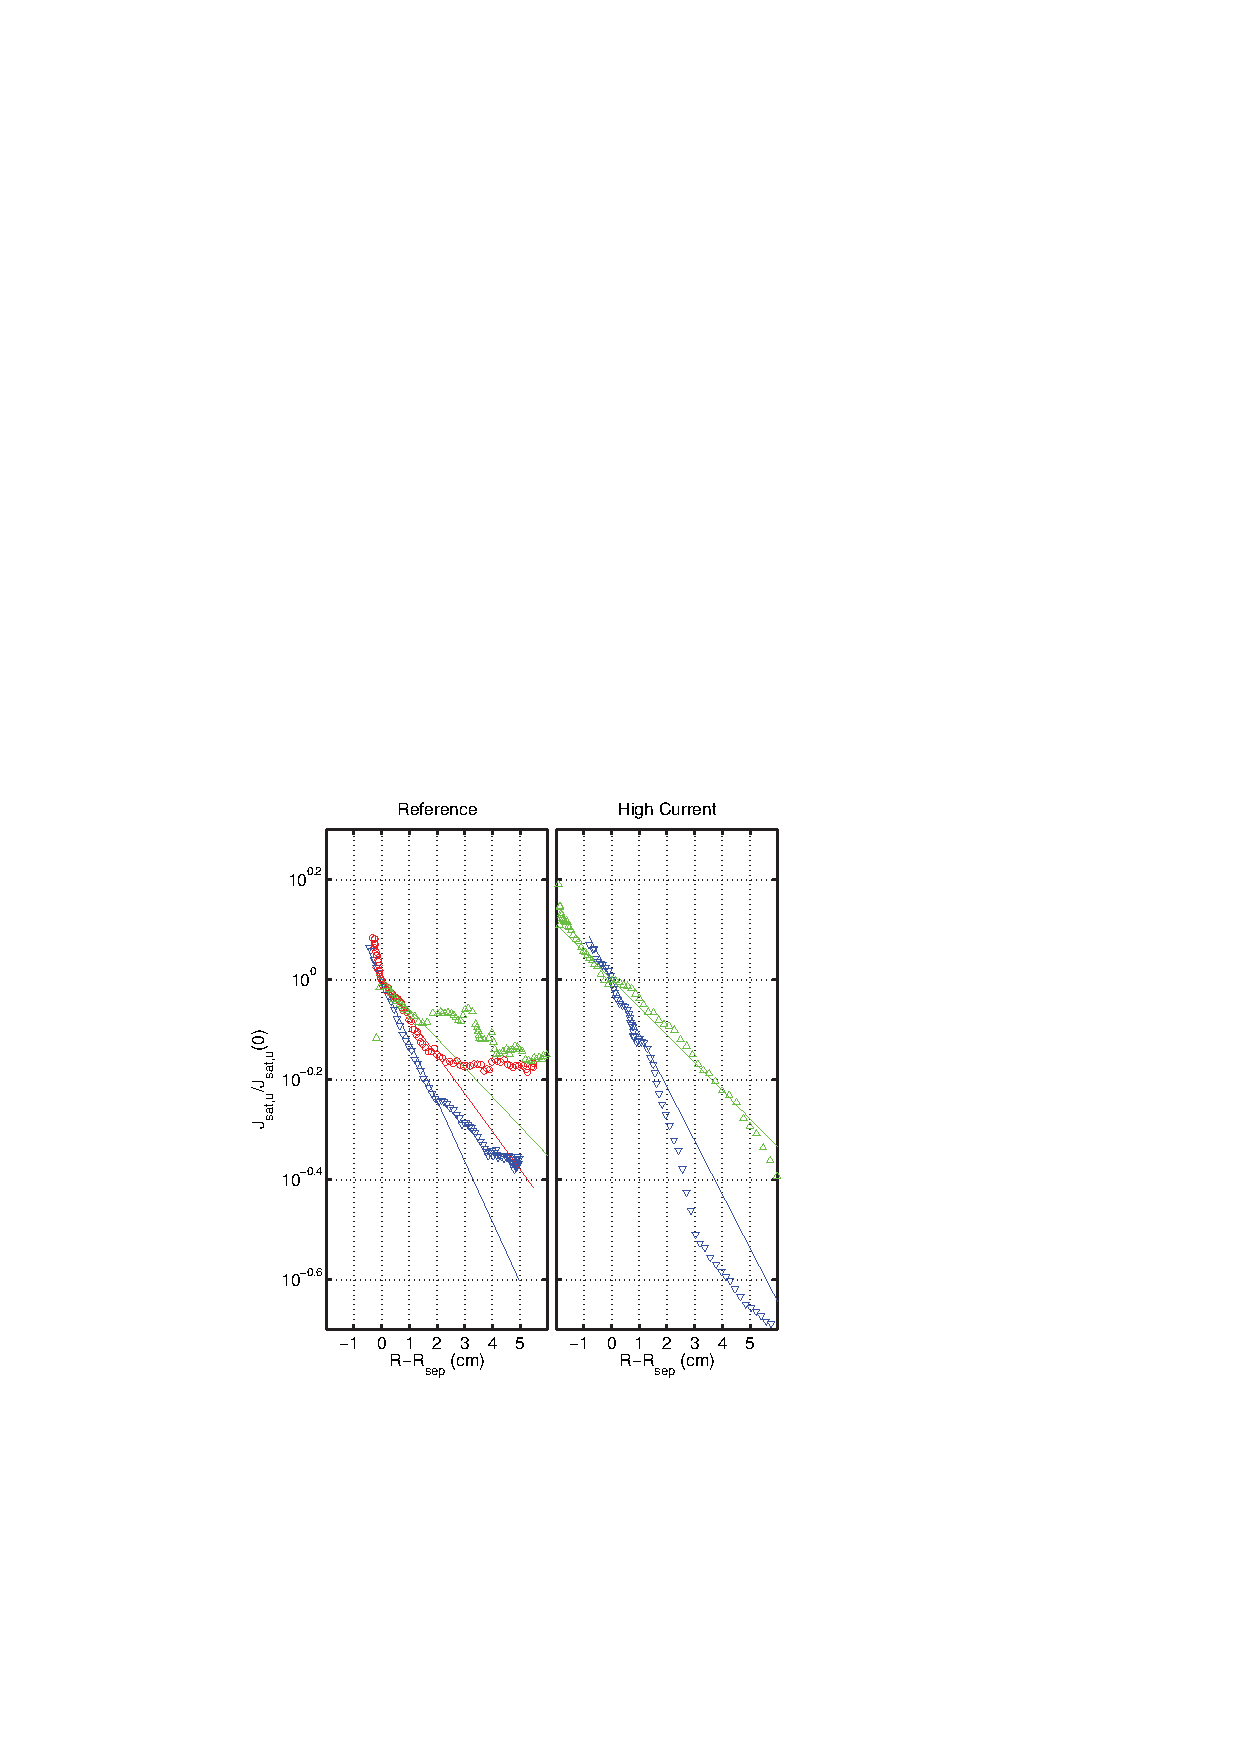
\includegraphics[width=\textwidth]{../pdfbox/Presentation/FigMilitello.pdf}
%     \end{column}
%   \end{columns}
% }
% \centering{\includegraphics<1>[width=1.1\textwidth]{../pdfbox/Presentation/Fig1Presentation}}
% \end{frame}

% \begin{frame}{Flux expansion scan/1}
% \vspace{-1cm}
%   \Fontvi
%   % \begin{columns}
%   %   \begin{column}{0.3\textwidth}
%       \centering{\includegraphics[width=.75\textwidth]{../pdfbox/Fig1a}}
%       \begin{itemize}
%       \item Parallel connection length varied by scanning 
%         flux expansion during density
%         ramps in ohmically heated discharges. \textcolor{red}{$\nabla B_i$ towards the X-point}
%         %\begin{equation*}
%         \[  f_x = \frac{(B_p/B_t)_{MP}}{(B_p/B_t)_{SP}}\]
%         %\end{equation*}
%         \item Variation of $f_x$ change the volume of flux tube as
%           well as parallel connection length (Increased up to 70\%)
%       \end{itemize}
%     % \end{column}
%     % \begin{column}{0.7\textwidth}
%   %   \end{column}
%   % \end{columns}
% \end{frame}

% \begin{frame}{Flux expansion scan/2}
%   \Fontvi
%       \begin{itemize}
%       \item<1-> Flux expansion variation induce modification at the target
%       \item<1-> Radiation front from bolometry  moves earlier in
%         density at larger f$_x$. Front movement trails CIII cut-off
%         movement (Reimerdes IAEA 2016)
%       \item<2-> Volumetric recombination rates from $n=6, 7$ balmer line
%         emission \parencite{kevin:jnm} indicates that \textcolor{red}{recombination occurs
%           earlier in density at high $f_x$}
%       \item<3|only@3> \textcolor{ta3skyblue}{This is not confirmed in reversed B$_t$ where
%         increasing the f$_x$ lead to deeper detachment without}
%         changing density threshold  
%     \end{itemize}
%     \only<1-2>{\begin{tikzonimage}[width=\textwidth]{../pdfbox/Fig2c}
%       \only<1>{\fill[white] (0.,0) rectangle (0.52,1); }    
%       \draw [->, ultra thick, black] (0.79,0.69) -- (0.75,0.51);
%     \end{tikzonimage}}
% \centering{\includegraphics<3>[width=.5\textwidth]{../pdfbox/Presentation/XD_detach_HM}}
%   \end{frame}

% \begin{frame}{Flux expansion scan/3}
%   \vspace{-1cm}
% \Fontvi
%       \begin{itemize}
%       \item Target and upstream profile measured at the same density
%         but different f$_x$
%       \item<3-> Target profiles in the near SOL modified with broader profile at higher
%         f$_x$. \textcolor{red}{Huge variation on $\Lambda_{div}$
%           without upstream modification}
%       \item<4|only@4> \textcolor{ta3chameleon}{Only further increase
%           of density (although $\Lambda_{div}$ in the far SOL
%           decreases) leads to profile broadening}
%       \end{itemize}
%       \centering{\includegraphics<1>[width=.65\textwidth]{../pdfbox/Fig4Series_1}}
%       \centering{\includegraphics<2>[width=.65\textwidth]{../pdfbox/Fig4Series_2}}
%       \centering{\includegraphics<3>[width=.65\textwidth]{../pdfbox/Fig4Series_3}}
%       \centering{\includegraphics<4>[width=.65\textwidth]{../pdfbox/Fig4Series_4}}
% \end{frame}

% \begin{frame}{Filaments effect}
%   \vspace{-1cm}
% \Fontvi
%       \begin{itemize}
%       \item<1-3> Blob properties deduced from fast reciprocating as done in \parencite{Boedo:2001tt}
%       \item<1|only@1> Blob size deduced as $\delta_b = \tau_b v_{\perp}$
%         % \begin{equation*}
%         %   \tau_b = \text{FWHM of CAS} \qquad v_{\perp} = \sqrt{v_{E\times B, r}^2 +
%         %     v_{E\times B, p}^2}
%         % \end{equation*}
%       \item<2-3> No clear dependence on
%           $\Lambda_{div}$ during f$_x$ scan
%       \item<3> \textcolor{ta3chameleon}{When we increase the
%           density filaments are bigger at same $\Lambda_{div}$}
%       \item<4-> \textcolor{ta3skyblue}{On a statistical basis,
%           blob size increases with density without clear dependence on
%           f$_x$ \onslide<5>{\textcolor{red}{as well as $\lambda_n$ in the Far SOL}}}
%       \item<6> \textcolor{ta3chameleon}{Behavior at very high
%           density to be confirmed}  
%       \end{itemize}
%       \centering{\includegraphics<1>[width=.53\textwidth]{../pdfbox/Fig14b}}
%       \centering{\includegraphics<2>[width=.63\textwidth]{../pdfbox/Fig7}}
%       \centering{\includegraphics<3>[width=.63\textwidth]{../pdfbox/Fig7b}}
%       \centering{\includegraphics<4>[width=.85\textwidth]{../pdfbox/Fig12}}
%       \centering{\includegraphics<5>[width=.85\textwidth]{../pdfbox/Fig12b}}
%       \only<6>{
%         \begin{center}
%           \begin{tikzonimage}[width=.85\textwidth]{../pdfbox/Fig12b}
%           \draw [thick, ta3chameleon, thick] (0.75,0.5) ellipse (0.1 and 0.1);
%           \end{tikzonimage}
%         \end{center}
%       }
% \end{frame}

% \begin{frame}{Current scan/1}
%   \begin{columns}
%     \begin{column}{0.5\textwidth}
%       \begin{itemize}
%       \item<1-3> On a single shape (f$_x \approx 4$) current scan with
%         similar density ramps performed
%       \item<2-3> \textcolor{red}{At lower current indication of shoulder for $R-R_{sep}
%         \geq 1$ cm which disappear at higher current (same density)}
%       \item<3> \textcolor{ta3chameleon}{At even higher current we need to substantially
%         increase the fueling (even if at the same $n/n_G$)}
%       \end{itemize}
%     \end{column}
%     \begin{column}{0.5\textwidth}
%       \only<1-2>{
%       \begin{tikzonimage}[width=\textwidth]{../pdfbox/Fig4d_series1}
%         \only<2>{
%           \draw [thick, red, thick] (0.75,0.75) ellipse (0.2 and 0.1);
%         }
%       \end{tikzonimage} }
%     \only<3>{
%       \begin{tikzonimage}[width=\textwidth]{../pdfbox/Fig4d_series2}
%           \draw [thick, ta3chameleon, thick] (0.67,0.35) ellipse (0.22 and 0.1);
%           \draw [thick, ta3chameleon, thick] (0.5,0.14) ellipse (0.3 and 0.03);
%         \end{tikzonimage}      
%       }
%     \end{column}
%   \end{columns}
% \end{frame}

% \begin{frame}{Current scan/2}
%   \begin{columns}
%     \begin{column}{0.5\textwidth}
%       \begin{itemize}
%       \item On a statistical basis we have a slight
%         reduction of radial velocity of the filaments as in MAST \parencite{Kirk:2016jj} with unclear
%         effect on blob-size
%       \end{itemize}
%     \end{column}
%       \begin{column}{0.5\textwidth}
%      \begin{tikzonimage}[width=\textwidth]{../pdfbox/Fig8}
%        \draw [->, ultra thick, red, dashed] (0.33,0.37) -- (0.7,0.27);
%      \end{tikzonimage}
%    \end{column}
%   \end{columns}
%   \end{frame}

% \begin{frame}{Lower Single Null (LSN) and Double Null (DN)}
%   \begin{columns}
%     \begin{column}{0.5\textwidth}
%       \begin{itemize}
%       \item<1|only@1> We compare LSN \textit{vs} DN on a single discharge at
%         two levels of density
%         \item<2|only@2> At lower density values the radiation is spread among
%           upper and lower X-points, whereas at higher density radiation
%           is higher at lower X-point
%         \item<6|only@6> Blob size increases with density with DN cases always
%           exhibiting larger blobs. Still compatible with general density
%           scaling. \textcolor{orange}{Radial velocity seems to decrease for DN}
%       \end{itemize}
%     \end{column}
%     \begin{column}{0.5\textwidth}
%       \includegraphics<1>[trim={0 7.6cm 0 0}, clip, width=\textwidth]{../pdfbox/Fig5}
%       \includegraphics<2>[width=\textwidth]{../pdfbox/Fig5c}
%       \only<6>{
%         \begin{tikzonimage}[width=\textwidth]{../pdfbox/Fig9}
%           \draw [->, thick, orange] (0.33, 0.33) -- (0.83, 0.21);
%         \end{tikzonimage}
%       }
%     \end{column}
%   \end{columns}
%   \only<3>{
%     \begin{itemize}
%       \item At the LFS target, DN density profile at lower level of
%         density is reduced and closer to 
%         what observed at higher density
%       \end{itemize}
%       \begin{tikzonimage}[width=\textwidth]{../pdfbox/Fig5e}
%         \draw [dashed, red, ultra thick] (0.7, 0.37) -- (0.3, 0.37);
%         \draw [->, dashed, red, ultra thick] (0.3, 0.7) -- (0.3, 0.38);
%       \end{tikzonimage}
%     }
%   \only<4-5>{
%     \begin{itemize}
%       \item Upstream profile suggests that a stronger tendency of
%         developing density shoulder is observed in DN 
%       \end{itemize}
%       \begin{tikzonimage}[width=\textwidth]{../pdfbox/Fig5d}
%         \only<5>{\draw[dashed, red, thick] (1.0, 0.55) -- (0.1, 0.55);}
%       \end{tikzonimage}
%     }

% \end{frame}

% \begin{frame}{Upper, Lower and Double Null}
%     \Fontvi
%     \begin{itemize}
%       \item The same density ramp performed in Upper, Lower and Double
%         null with all the Strikes points at the inner wall
%       \item This allow to test any possible dependence from $\nabla
%         B_i$ drift direction. C-Mod suggests difference in the medium
%         density range \parencite{LaBombard:2004kg}
%     \end{itemize}
%     \centering{\includegraphics[width=0.9\textwidth]{../pdfbox/Fig1b}}
% \end{frame}
% \begin{frame}{Upper, Lower and Double Null}
%     \Fontvi
%     \begin{itemize}
%       \item<2-> Lower and Double null blob size scale consistently with
%         density scaling
%       \item<3->  Upper Single null always exhibits
%         larger blob
%       \end{itemize}
%       \vspace{-0.27cm}
%     \centering{\includegraphics<1>[width=.6\textwidth]{../pdfbox/Fig11b_Series1}}
%     \centering{\includegraphics<2>[width=.6\textwidth]{../pdfbox/Fig11b_Series2}}
%     \centering{\includegraphics<3>[width=.6\textwidth]{../pdfbox/Fig11b_Series3}}
% \end{frame}  

% \begin{frame}{Summary}
%   \Fontvi
%   \begin{itemize}
%   \item<1-> $\lambda_n = |\nabla n_e/n_e|^{-1}$ computed around 1cm from the
%     separatrix
%   \item<2-> $\lambda_n$ clearly increases with $\Theta = (\delta_b
%         R^{1/5}/L_{\parallel}^{2/5}\rho_s^{4/5})^{5/2}$,
%     i.e. with blob-size
%   \item<3-> \alert{The dependence on L$_{\parallel}$ is marginal
%       although we obtain 
%       larger $\Theta$ at smaller $L_{\parallel}$}.
%   \item<4-> The increase of $\lambda_n$ is consistent with an increase
%     of perpendicular to parallel losses
%   \item<5-> The dependence on $\Lambda_{div}$ is weaker than in
%     AUG/JET. \onslide<6>{\textcolor{ta3chameleon}{ Large $\Lambda$ is not
%         sufficient for flat profile.}}
      
%   \end{itemize}
%   \begin{tikzonimage}[width=\textwidth]{../pdfbox/Fig10c}
%     \only<1>{\fill[white] (0, 0) rectangle (1, 1);}
%     \only<2>{\fill[white] (0.348,0) rectangle (1,1); }    
%     \only<3>{\fill[white] (0.348,0) rectangle (0.897,1); }    
%     \only<4>{\fill[white] (0.62,0) rectangle (0.897,1); }    
%     \only<6>{
%       \draw [thick, ta3chameleon, thick, rotate = 4] (0.865,0.2) ellipse (0.04 and 0.2);
%       \draw [thick, ta3chameleon, thick, rotate = 3] (0.72,0.6) ellipse (0.03 and 0.15);
%  }    
%     \end{tikzonimage}
% \end{frame}

\end{document}
%\draw [thick, blue, thick, rotate=-4] (0.8,0.55) ellipse (0.1 and 0.33);
